\documentclass[12pt,twoside]{mitthesis}

%%%%%%%%%%%%%%%%%%%%%%%%%%%%%%%%%%%%%%%%%%%%%%%%%%%%%%%%%%%%%%%%%%%%%%%%%%%%%%%%
% PREAMBLE

\usepackage[bitstream-charter]{mathdesign} % Use BT Charter font
\usepackage[T1]{fontenc}                   % Use T1 encoding instead of OT1
\usepackage[utf8]{inputenc}                % Use UTF8 input encoding
\usepackage{microtype}                     % Improve typography
\usepackage{amsmath}                       % AMS Math extensions
\usepackage{booktabs}                      % Improve table spacing
\usepackage{graphicx}                      % Extended graphics capabilities
\usepackage{tocbibind}                     % Include listings in TOC
\usepackage[printonlyused]{acronym} % withpage: for showing page of use
\usepackage{listings}                      % Source code listings
\usepackage{caption}
\usepackage{subcaption}
\usepackage[rgb]{xcolor}
\usepackage{url}
\usepackage{array}
\usepackage{pdfpages}
\usepackage{mathtools}
\usepackage{setspace}
\usepackage{pbox}
\usepackage{tikz}
\usetikzlibrary{calc,shapes,decorations.pathreplacing,positioning}
\usepackage{pgfplots}

\usepackage[breaklinks=true]{hyperref}
\hypersetup{colorlinks=true, linkcolor=black, citecolor=black, urlcolor=black,
  pdftitle={Domain Decomposition for Monte Carlo Particle Transport Simulations
  of Nuclear Reactors},
  pdfauthor={Nicholas Edward Horelik}
}
\pagestyle{plain}

%\usepackage{floatrow}
%\floatsetup[table]{style=plaintop}
%\floatsetup[widefigure]{margins=hangleft}

% Appendix
\usepackage[toc,page]{appendix}

% Don't reset footnote counter between chapters
\usepackage{chngcntr}
\counterwithout{footnote}{chapter}

% Algorithm constructs
\usepackage[chapter]{algorithm} % Provides algorithm environment
\usepackage{algorithmicx}       % Provides algorithmic block
\usepackage{algpseudocode}      % Option of algorithmicx package
\renewcommand{\thealgorithm}{\thechapter-\arabic{algorithm}}
\newcommand\Algphase[1]{%
\vspace*{-.7\baselineskip}\Statex\hspace*{\dimexpr-\algorithmicindent-2pt\relax}\rule{\columnwidth}{0.4pt}%
\Statex\hspace*{-\algorithmicindent}{#1}%
\vspace*{-.7\baselineskip}\Statex\hspace*{\dimexpr-\algorithmicindent-2pt\relax}\rule{\columnwidth}{0.4pt}%
}
\newcommand{\algrule}[1][.4pt]{\par\vskip.5\baselineskip\hrule height #1\par\vskip.5\baselineskip}

% Configure captions
\captionsetup{labelfont=bf, labelsep=colon}
\captionsetup[algorithm]{labelfont=bf, labelsep=colon}

% Use Latin Modern for typewriter fonts
\renewcommand{\ttdefault}{lmtt}

% Add \unit macro
\newcommand{\unit}[1]{\ensuremath{\, \mathrm{#1}}}

\definecolor{gray}{rgb}{0.4,0.4,0.4}
\definecolor{darkblue}{rgb}{0.0,0.0,0.6}
\definecolor{cyan}{rgb}{0.0,0.6,0.6}
\lstset{
  basicstyle=\footnotesize\ttfamily,
  columns=fullflexible,
  showstringspaces=false,
  commentstyle=\color{gray}\upshape,
  frame=single,
  xleftmargin=0.55in
}

\lstdefinelanguage{XML}
{
  morestring=[b]",
  morestring=[s]{>}{<},
  morecomment=[s]{<?}{?>},
  morecomment=[s]{<!--}{-->},
  stringstyle=\color{black},
  identifierstyle=\color{darkblue},
  keywordstyle=\color{cyan},
  morekeywords={}
}

\setcounter{secnumdepth}{4}
\setcounter{tocdepth}{3}

\renewcommand{\contentsname}{Table of Contents}
\renewcommand{\bibname}{References}

\begin{document}

%%%%%%%%%%%%%%%%%%%%%%%%%%%%%%%%%%%%%%%%%%%%%%%%%%%%%%%%%%%%%%%%%%%%%%%%%%%%%%%%
% TITLE PAGE

\title{Reactor Agnostic Cross-Section Generation for Fine-Mesh Deterministic Neutron Transport Simulations}

\author{William Robert Dawson Boyd III}
\prevdegrees{B.S., Georgia Institute of Technology (2010) \\
             M.S., Massachusetts Institute of Technology (2014)}
\department{Department of Nuclear Science and Engineering}
\degree{Doctor of Philosophy in Nuclear Science and Engineering}

\degreemonth{September}
\degreeyear{2016}
\thesisdate{September 1, 2016}

\supervisor{Benoit Forget}{Associate Professor of Nuclear Science and Engineering}
\reader{Kord S. Smith}{KEPCO Professor of the Practice of Nuclear Science and Engineering}
\chairman{Emilio Bagglietto}{Associate Professor of Nuclear Science and Engineering}

%\includepdf{signed-cover-page.pdf}
%\maketitle

%%%%%%%%%%%%%%%%%%%%%%%%%%%%%%%%%%%%%%%%%%%%%%%%%%%%%%%%%%%%%%%%%%%%%%%%%%%%%%%
% ABSTRACT

\cleardoublepage
\setcounter{savepage}{\thepage}

\begin{abstractpage}

The development of high fidelity multi-group neutron transport-based simulation tools for full core Light Water Reactor (LWR) analysis has been a long-standing goal of the reactor physics community. While direct transport simulations have previously been far too computationally expensive, advances in computer hardware have allowed large scale simulations to become feasible. Therefore, many have focused on developing full core neutron transport solvers that do not incorporate the approximations and assumptions of traditional nodal diffusion solvers. 

Due to the computational expense of direct full core 3D deterministic neutron transport methods, many have focused on 2D/1D methods which solve 3D problems as a coupled system of radial and axial transport problems. However, the coupling of radial and axial problems also introduces approximations. Instead, the work in this thesis focuses on explicitly solving the 3D deterministic neutron transport equations with the Method of Characteristics (MOC).

MOC has been widely used for 2D lattice physics calculations due to its ability to accurately and efficiently simulate reactor physics problems with explicit geometric detail. The work in this thesis strives to overcome the significant computational cost of solving the 3D MOC equations by implementing efficient track generation, axially extruded ray tracing, Coarse Mesh Finite Difference (CMFD) acceleration, linear track-based source approximations, and scalable domain decomposition. 

Additionally, significant attention has been be given to complications that arise in full core simulations with transport-corrected cross-sections. The convergence behavior of transport methods is analyzed, leading to a new strategy for stabilizing the source iteration scheme for neutron transport simulations. The methods are incorporated into the OpenMOC reactor physics code and simulation results are presented for the full core BEAVRS LWR benchmark. Parameter refinement studies and comparisons with reference OpenMC Monte Carlo solutions show that converged full core 3D MOC simulations are feasible on modern supercomputers for the first time.

%However, 3D full core LWR simulations present significant challenges due to greatly increased computational cost.

%The Method of Characteristics (MOC) has seen wide interest in reactor physics because of its accuracy and efficiency in computing lattice physics problems. While most of its use has been in solving 2D problems, there has been recent interest in extending MOC to 3D in order to more accurately calculate 3D power distributions in LWRs. While the method is naturally extensible to 3D, it presents significant computational difficulties. Methods will be presented which mitigate the computational difficulties of 3D MOC by using domain decomposition, efficient track generation, axially extruded ray tracing, CMFD acceleration, and a linear source approximation. Significant attention will be given to complications that arise in full core simulations. 3D MOC results will be presented for the full core simulation of the BEAVRS benchmark, showing that 3D MOC can be a viable tool for anal

\end{abstractpage}

\cleardoublepage

%%%%%%%%%%%%%%%%%%%%%%%%%%%%%%%%%%%%%%%%%%%%%%%%%%%%%%%%%%%%%%%%%%%%%%%%%%%%%%%
% ACKNOWLEDGMENTS

\section*{Acknowledgments}

This work was supported by the Office of Advanced Scientific Computing Research,
Office of Science, US Department of Energy, under Contract DE-AC02-06CH11357.

\pagestyle{plain}

%%%%%%%%%%%%%%%%%%%%%%%%%%%%%%%%%%%%%%%%%%%%%%%%%%%%%%%%%%%%%%%%%%%%%%%%%%%%%%%
% TABLE OF CONTENTS, FIGURES, TABLES

\begin{singlespace}
\tableofcontents
\newpage
\listoffigures
\newpage
\listoftables
\listofalgorithms
\addcontentsline{toc}{chapter}{List of Algorithms}
\newpage
\section*{Definitions and Acronyms}

\begin{acronym}[TDMA,smaller]
  \acro{API}{Application Programming Interface}
  \acro{BWR}{Boiling Water Reactor}
  \acro{BEAVRS}{Benchmark for Evaluation and Validation of Reactor Simulations}
  \acro{CASL}{Consortium for Advanced Simulation of \acp{LWR}}
  \acro{CESAR}{Center for Exascale Simulation of Advanced Reactors}
  \acro{CSG}{Constructive Solid Geometry}
  \acro{CMFD}{Coarse Mesh Finite Difference}
  \acro{FSR}{Flat Source Region}
  \acro{HPC}{High-Performance Computing}
  \acro{IFBA}{Integral Fuel Burnable Absorbers}
  \acro{LNS}{Local Neighbory Symmetry}
  \acro{LWRs}{Light Water Reactors}
  \acro{MC}{Monte Carlo}
  \acro{MCPR}{Minimum Critical Power Ratio}
  \acro{MGXS}{Multi-Group Cross Sections}
  \acro{MOC}{Method of Characteristics}
  \acro{MPI}{Message Passing Interface}
  \acro{PCM}{per cent mille}
  \acro{PWR}{Pressurized Water Reactor}
  \acro{SPH}{SuPerHomogenisation Factors}
  \acro{TRISO}{TRistructural-ISOtropic}
  \acro{VHTR}{Very High Temperature Reactor}
\end{acronym}

\addcontentsline{toc}{chapter}{Definitions and Acronyms}
\end{singlespace}

%%%%%%%%%%%%%%%%%%%%%%%%%%%%%%%%%%%%%%%%%%%%%%%%%%%%%%%%%%%%%%%%%%%%%%%%%%%%%%%
% CHAPTERS

\chapter{Introduction}
\label{chap:intro}

%%%%%%%%%%%%%%%%%%%%%%%%%%%%%%%%%%%%%%%%%%%%%%%%%%%%%%%%%%%%%%%%%%%%%%%%%%%%%%%
\section{Motivation}
\label{sec:chap1-motivation}

%Intro paragraph\\
%-talk about the increasingly important role of simulation in nuclear?\\
%-challenges for today's nuclear fleet which simulation is well-poised to tackle\\
%-segue into talk about nuclear reactor / neutron physics paragraph\\
%-based on empirical models\\
%-need to account for angular dependence of neutron flux (e.g. "transport" methods)\\

Numerical simulation has long played an important role in nuclear reactor physics and engineering. The nuclear industry relies on computational modeling of the neutron physics in reactors to predict core reactivity, power distributions, fuel depletion, and transient behavior to ensure the safety and reliability of the current fleet of Light Water Reactors (LWRs). Predictive simulations are necessary to evaluate innovations which seek to improve reactor safety and fuel cycle economics, such as reduced safety margin uncertainties, accident-tolerant fuels, and extended cycle lengths. In addition, simulation is used to assess the technical competencies of advanced reactor technologies such as Small Modular Reactors (SMRs), Sodium Fast Reactors (SFRs), Molten Salt Reactors (MSRs), High Temperature Gas Reactors (HTGRs), among other proposed designs. 

Many Generation III+ reactors, such as the Westinghouse AP1000\texttrademark \ac{PWR}, optimize performance with complicated core designs. A variety of reactivity control mechanisms -- including partially-inserted control rods, ``grey'' control poisons, \ac{IFBA}, soluble boron, etc. -- along with axial enrichment zoning are used to improve performance metrics such as power peaking factors. The reactor analysis methods in widespread use today assume a ``smoothly'' varying flux distribution, and are not well-suited to model highly localized flux gradients which result from these complex core configurations. New high-fidelity simulation tools are needed to accurately capture neutron physics in advanced reactor designs.

The development and deployment of neutron physics simulations is governed by tradeoffs between accuracy and speed. High-fidelity simulations are accurate and flexible since they make few approximations, but they require significant computational time and resources. On the other hand, the assumptions and approximations made by low-fidelity methods enable optimizations which greatly improve the time-to-solution. However, low-fidelity models are designed for specific applications and lose their predictive power when employed in settings outside of the scope for which they were intended. As a result, it is common to employ a mix of high- and low-fidelity tools for reactor analysis -- for example, high-fidelity tools are frequently used to inform and benchmark low-fidelity models for use within a narrow envelope of design paramters. This thesis develops a new approach within the same vein by employing continuous energy Monte Carlo neutron transport simulations to generate accurate multi-group cross sections for computationally efficient fine mesh deterministic transport methods.


%%%%%%%%%%%%%%%%%%%%%%%%%%%%%%%%%%%%%%%%%%%%%%%%%%%%%%%%%%%%%%%%%%%%%%%%%%%%%%%
\section{Background}
\label{sec:chap1-background}

A key trend in recent years has been the steady progress towards whole-core neutron transport-based reactor analysis tools. The standard methods used for reactor analysis today continue to be based on diffusion theory, which enables orders of magnitude computational performance improvements with respect to transport methods. Diffusion-based methods coupled with accurately modeled cross section data have proven to be sufficiently accurate for software tools used by reactor analysts, designers and regulators in industry and academia. However, these techniques rely on a number of assumptions and approximations which are not valid for all reactor types. For example, some Generation IV reactor design concepts are significantly more challenging to model than \ac{LWR}s due to the high degree of spectral coupling between geometrically disparate zones within the core. Although the computational requirements for whole-core transport-based simulations have precluded their widespread deployment, the continuing growth of cheap parallel processing power has made the prospects for such tools increasingly feasible.

%Transport-based methods would enable more accurate core power distributions to be calculated without the approximations needed for today’s tools based upon diffusion theory.

\ac{MC} particle transport methods are often looked to as the ``gold standard'' for the future of nuclear reactor core depletion calculations. Monte Carlo methods are by their very nature \textit{reactor agnostic} in that they permit an accurate treatment of the core geometry and spectral coupling. Another appealing characteristic of \ac{MC} methods is their ability to use continuous energy cross sections with up to tens of thousands of energy points. An accurate treatment of evaluated cross section data permits high-fidelity core spectral calculations. Although new scalable parallel algorithms have enabled codes to achieve excellent scaling on 100,000s of cores, production tools for industrial workstations remain out of reach for the foreseeable future. The primary reason for this is that the inverse square root convergence rate inherent to \ac{MC} makes it computationally intractable to realize an acceptably low uncertainty for each tally of interest except on large supercomputers. Furthermore, whole-core Monte Carlo calculations require a terabyte of memory or more to store the tallied quantities, which is inaccessible except on the world's largest computing machines. Finally, the accurate energy treatment largely renders \ac{MC} methods inefficient for modern computational hardware. The stochastic treatment of the nonlinear neutron energy characterization is challenging to vectorize and results in highly disjoint memory accesses to cross section data with minimal cache reuse. 

An attractive alternative to MC are deterministic methods -- such as Discrete Ordinates (S$_N$), Simplified P$_N$ (SP$_N$), and the Method of Characteristics (MOC). Deterministic methods typically do not make use of continuous energy cross section data and instead discretize the energy domain through the multi-group energy approximation as shown in Fig.~\ref{fig:chap1-u235-sigf}. The multi-group approximation considerably reduces the necessary dataset footprint for simulation. In addition, the multi-group approximation enables deterministic methods to be more readily formulated in such a way as to permit greater vectorization and cache reuse than \ac{MC} methods. However, the approximation requires an \textit{a priori} estimate of the neutron flux to compute the \ac{MGXS} in each energy group and spatial zone in order to solve for the flux distribution throughout the core.

\begin{emphbox}
\textbf{This thesis is motivated by the desire to obtain Monte Carlo-quality solutions with computationally efficient deterministic neutron transport methods.}
\end{emphbox}

%Deterministic transport methods pose a number of advantages to \ac{MC} from a computational perspective, which seems likely to make these methods more viable in the near to intermediate term. However, deterministic methods almost universally discretize the energy domain in a few to hundreds of energy groups. This approximation requires energy condensed \ac{MGXS} in each geometric region to preserve reaction rates.

\begin{figure}
\centering
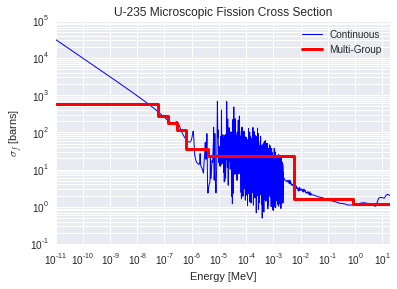
\includegraphics[width=0.8\linewidth]{figures/intro/u235-ce-mg-xs}
\caption[U-235 continuous energy and multi-group fission cross section]{U-235 continuous energy and 16-group fission cross section.}
\label{fig:chap1-u235-sigf}
\end{figure}

Many different engineering prescriptions have been developed to generate \ac{MGXS} for specific reactor configurations and spectra. In general, \ac{MGXS} generation schemes use a multi-level approach to decouple the energy, angular and spatial dimensions as depicted in Fig.~\ref{fig:chap1-multi-level-flow-chart}. The multi-level approach typically applies high-fidelity models of the energy self-shielding physics to low-fidelity geometric models of unique core components. The complexity of the energy treatment is then reduced at each level as larger and more complex geometric models are considered.

\begin{figure}
\centering
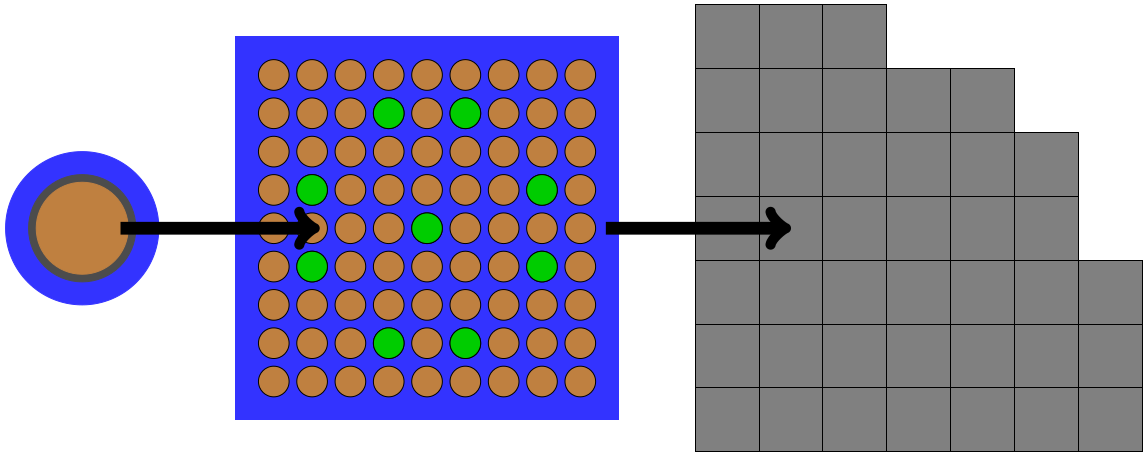
\includegraphics[width=0.9\linewidth]{figures/intro/multi-step-flow-chart}
\caption[Multi-level approach to reactor analysis]{Current multi-level framework for reactor analysis.}
\label{fig:chap1-multi-level-flow-chart}
\end{figure}

For example, the first stage for \ac{LWR} \ac{MGXS} generation attempts to capture energy self-shielding effects within simplified geometric models such as infinite fuel pin cells. This step typically condenses continuous energy cross sections to $\mathcal{O}(100)$ groups. These \ac{MGXS} are then used in a heterogenous lattice physics calculation of an individual fuel assembly within an infinite lattice. The lattice physics calculation models spatial self-shielding effects between pins of various material compositions and condenses the \ac{MGXS} to a coarse energy structure of $\mathcal{O}(10)$ groups. In addition, the \ac{MGXS} may be spatially-homogenized across the entire fuel assembly or across each fuel pin within each assembly. Finally, the spatially-homogenized coarse \ac{MGXS} for each fuel assembly are used in a whole-core calculation composed of many fuel assemblies.

The multi-level approach uses a combination of models of varying complexity to optimize overall simulation speed with accuracy. However, this is typically done at the sake of generality. For example, some prior knowledge of the neutron energy spectra is required to design approximations to the flux for a particular reactor configuration. Furthermore, multi-level \ac{MGXS} generation schemes do not generally model inter-assembly physics or the effect of reflectors and other core heterogeneities on the spatial distribution of the flux. Instead, geometric heuristcs are often used to embed spatial self-shielding effects in \ac{MGXS} for similarly shielded spatial zones (\textit{e.g.}, fuel pins). The approximations to the energy and spatial variation of the flux introduce approximation error in whole-core calculations and limit the space of core design parameters for which multi-level schemes may be applied. New reactor agnostic \ac{MGXS} generation methods are needed to enable deterministic transport-based methods to be as accurate and flexible as Monte Carlo in whole-core calculations.

%For reactors with a greater degree of spectral coupling, however, these approximations are not valid, resulting in ever larger datasets for the cross section generation process.

This thesis investigates the use of Monte Carlo methods to generate \ac{MGXS} for whole-core deterministic reactor analyis. Monte Carlo presents a natural approach to replace engineering prescriptions to approximate the flux with a stochastic approximation of the exact flux. The advantage of a \ac{MC}-based approach is that all of the relevant physics modeled in \ac{MC} may be directly embedded into \ac{MGXS}. This improvement in accuracy comes at the computational expense of converging group constant tallies to acceptably low uncertainties. \ac{MC} methods have increasingly been used to generate few group constants for coarse mesh diffusion, most notably by the Serpent \ac{MC} code~\cite{serpent2013manual}. However, there exist few rigorous and comprehensive analyses of \ac{MGXS} generation for heterogeneous fine mesh deterministic transport methods. 

\begin{emphbox}
\textbf{This thesis develops and evaluates \ac{MC}-based methods to generate \ac{MGXS} for fine mesh deterministic neutron transport codes.}
\end{emphbox}

In addition, \ac{MC}-based \ac{MGXS} generation methods to date have retained the multi-level geometric framework to tabulate \ac{MGXS} for individual reactor components -- such as infinite fuel pins and/or assemblies -- for subsequent use in whole-core multi-group calculations. Although the use of \ac{MC} within a multi-level scheme eliminates the need to approximate the flux in energy, it is does not account for spatial self-shielding effects throughout a reactor core. This thesis abandons the multi-level framework in place of a whole-core \ac{MC} calculation which simultaneously accounts for all energy and spatial self-shielding effects in a single step.

In theory, whole-core \ac{MC} calculations can be used to tally \ac{MGXS} in each spatial zone (\textit{e.g.}, 50,000+ fuel pins in a \ac{PWR} core) to account for the spatial variation in the flux. However, such simulations have not been employed for practical reasons -- in particular, the large memory footprint and computational expense of performing such calculations has been prohibitive for \ac{MC} codes until recent years. Furthermore, roughly the same number of particle histories would be required to converge the \ac{MGXS} tallies in each spatial zone as would be required for a direct whole-core calculation by \ac{MC}. Hence, it would be more useful to simply use \ac{MC} to compute the solution to the whole-core eigenvalue problem directly rather than use it to fully embed spatial self-shielding effects in \ac{MGXS} for deterministic transport codes. Therefore, in order for \ac{MC} to be practical for reactor agnostic fine mesh \ac{MGXS} generation, a new method is required to accelerate the convergence rate of the \ac{MGXS} tallies in each fine mesh region to a degree that is not possible for conventional whole-core Monte Carlo simulations. 

This thesis proposes to use statistical clustering methods to accelerate the convergence rate of whole-core \ac{MC} calculations for \ac{MGXS} generation. The novel approach developed in this work relies on the fact that many distinct spatial zones across a reactor core will experience similar if not identical spatial self-shielding effects, and therefore have similar if not identical \ac{MGXS}. The stochastic nature of \ac{MC} simulations will contribute statistical ``noise'' to the tally estimates for the \ac{MGXS}. As a result, the \ac{MGXS} estimates for similarly self-shielded spatial zones will form clusters which will converge as more particle histories are simulated. The goal of this thesis is to develop and apply algorithms to identify \ac{MGXS} clusters from ``noisy'' Monte Carlo tally data and to predict the true mean of each cluster prior to convergence. This methodology aims to generate \ac{MGXS} for deterministic neutron transport codes in a reactor agnostic and computationally efficient manner.

%The true mean of each cluster will then be used as the predicted estimate for the multi-group cross-section for each fine-mesh region in each cluster.

\begin{emphbox}
\textbf{This thesis uses statistical clustering algorithms to accelerate whole-core \ac{MC} calculations
which simultaneously model all energy- and spatial self-shielding effects for fine mesh \ac{MGXS} generation.}
\end{emphbox}


%%%%%%%%%%%%%%%%%%%%%%%%%%%%%%%%%%%%%%%%%%%%%%%%%%%%%%%%%%%%%%%%%%%%%%%%%%%%%%%
\section{Thesis Objectives}
\label{sec:chap1-objectives}

The subject matter of this thesis is organized along two main themes:

\begin{itemize}
\item \textbf{\textit{Approximation Error}} -- Quantify and diagnose approximation error(s) in \ac{MGXS} generated from \ac{MC} methods for simple heterogeous benchmark problems.
\item \textbf{\textit{Statistical Clustering}} -- Develop statistical clustering methods to accelerate the convergence rate of \ac{MGXS} on heterogeneous \ac{MC} tally meshes.
\end{itemize}

The first theme of this thesis rigorously assesses the efficacy of \ac{MGXS} generation with \ac{MC} for fine mesh transport calculations. Some of the approximations made by \ac{MC}-based \ac{MGXS} generation are quantified, including the energy- and spatial-dependence of condensed \ac{MGXS}. An in-depth analysis of systematic bias resulting from constant-in-angle total \ac{MGXS} is presented, along with a scheme based on \ac{SPH} factors to compensate for this loss in accuracy. 

The second theme of this thesis develops a new methodology to simultaneously capture local and global spatial self-shielding effects in \ac{MGXS} for whole-core calcuations. This scheme applies statistical clustering methods to accelerate the convergence rate of \ac{MGXS} tallied on fine, heterogeneous spatial meshes in Monte Carlo. The latent variable model which inspires the clustering paradigm is presented, along with a discussion of the implementation of a data pipeline to evaluate clustering algorithms for \ac{MGXS} generation. A series of increasingly complex heterogeneous benchmarks are modeled to empirically compare the accuracy and convergence rate of the approach with more traditional multi-level schemes for \ac{MC}-based MGXS generation.


%%%%%%%%%%%%%%%%%%%%%%%%%%%%%%%%%%%%%%%%%%%%%%%%%%%%%%%%%%%%%%%%%%%%%%%%%%%%%%%
\section{Thesis Outline}
\label{sec:chap1-outline}

This thesis is segmented into five Parts. Part I is comprised of this introductory chapter.

Part II discusses the relevant background information for this thesis. Chap.~\ref{chap:mgxs} reviews multi-group neutron transport theory and considers some common approximations made in \ac{MGXS} generation and multi-group transport codes. Chap.~\ref{chap:mgxs-mc} introduces Monte Carlo as an approach to generate \ac{MGXS}, and highlights relevant studies in the literature which have used \ac{MC} to generate \ac{MGXS}. Chap.~\ref{chap:workflow} presents the simulation workflow developed for this thesis to evaluate \ac{MC} for \ac{MGXS} generation, including the OpenMC, OpenMOC and OpenCG codes.

Part III diagnoses common sources of approximation error in \ac{MGXS} generation and multi-group transport methods. Chap. \ref{chap:biases} quantifies the impact of multi-group approxmation error for simple, heterogeneous \ac{PWR} geometries. Chap.~\ref{chap:sph} presents an algorithmic approach to mitigate systematic biases resulting from constant-in-angle total \ac{MGXS} using \ac{SPH} factors, and motivates the need for future work to address this issue.

Part IV develops a novel approach based on statistical clustering methods to accelerate whole-core \ac{MC} calculations for \ac{MGXS} generation. Chap.~\ref{chap:benchmarks} analyzes the convergence rate of \ac{MGXS} datasets computed on fine spatial \ac{MC} tally meshes for a series of heterogeneous \ac{PWR} benchmark models to motivate this new methodology. Chap.~\ref{chap:quantify} quantifies the impact of using \ac{MGXS} which reflect inter-pin and inter-assembly spatial self-shielding effects on the solutions computed by multi-group deterministic transport methods. Chap.~\ref{chap:spatial} analyzes the emergence of \ac{MGXS} clusters due to spatial self-shielding with a variety of visual aids. Chap.~\ref{chap:unsupervised} outlines a latent variable model for clustering \ac{MGXS}, along with a data pipeline for unsupervised clustering to accelerate the \ac{MGXS} convergence rate. Chapter~\ref{chap:results} evaluates the impact of clustered \ac{MGXS} on the accuracy and convergence rate of the eigenvalue solutions computed by deterministic transport methods.

Part V is composed of Chapter~\ref{chap:conclusions} which summarizes the progress made in this thesis to chart a path forward for \ac{MC}-based \ac{MGXS} generation for whole-core deterministic transport methods.

%\begin{figure}
%\begin{subfigure}{\textwidth}
%  \centering
%  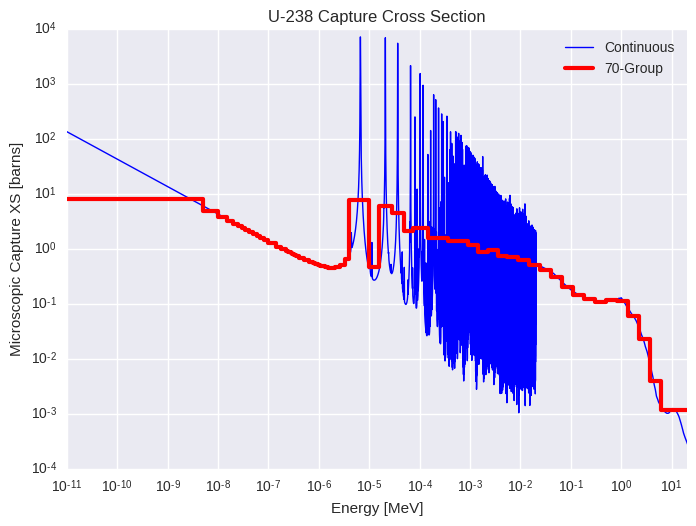
\includegraphics[width=0.9\linewidth]{figures/intro/u238-capture-70}
%  \caption{}
%\end{subfigure}
%\begin{subfigure}{\textwidth}
%  \centering
%  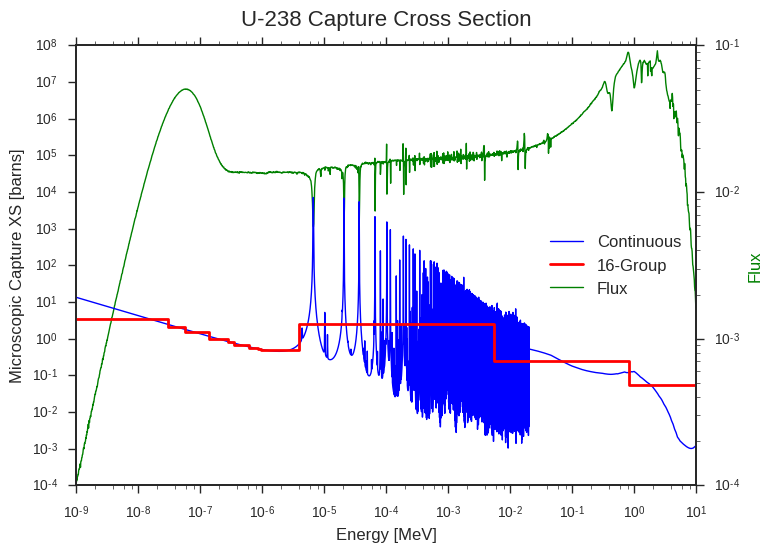
\includegraphics[width=0.9\linewidth]{figures/intro/u238-capture-16}
%  \caption{}
%\end{subfigure}
%\caption[Uranium-238 capture cross section]{Continuous energy and multi-group cross sections for U-238 capture in a PWR spectrum for 70-groups (a) and 16-groups (b).}
%\label{fig:pwr-ce-mg-xs}
%\end{figure}


\chapter{Domain Decomposition}
\label{chap:dd}

%%%%%%%%%%%%%%%%%%%%%%%%%%%%%%%%%%%%%%%%%%%%%%%%%%%%%%%%%%%%%%%%%%%%%%%%%%%%%%%%
%%%%%%%%%%%%%%%%%%%%%%%%%%%%%%%%%%%%%%%%%%%%%%%%%%%%%%%%%%%%%%%%%%%%%%%%%%%%%%%%
\section{Background}

The memory challenges discussed in Chapter~\ref{chap:intro} can be addressed
with \emph{domain decomposition}. We specifically focus on the spatial domain
because that is where the largest memory burdens are incurred: spatially
heterogeneous tallies and materials needed for full-core depletion. While many
nuances to the concept can be conceived, the core idea of domain
decomposition is easily conceptualized: distributed compute resources load
materials into memory for different subsections of the problem domain, and score
tally results for regions only within that domain.




\chapter{Full-Core Analysis}
\label{chap:full_core}

%%%%%%%%%%%%%%%%%%%%%%%%%%%%%%%%%%%%%%%%%%%%%%%%%%%%%%%%%%%%%%%%%%%%%%%%%%%%%%%%
%%%%%%%%%%%%%%%%%%%%%%%%%%%%%%%%%%%%%%%%%%%%%%%%%%%%%%%%%%%%%%%%%%%%%%%%%%%%%%%%
\section{Introduction}

The discussion thus far has focused on the performance of domain decomposition
from the perspective of particle communication and load imbalance penalties.
With an implementation that has minimized overhead as a result of these, we
should now have the ability to treat the full-core PWR problem with the desired
tally and material memory burdens. For this to be done efficiently, data
management algorithms should be designed with the full scale of the problem in
mind, such as the ones discussed. In
addition, careful attention must be paid to several practicalities related to
problem-specification and post-processing.

The size of the \ac{PWR} depletion problem was described.
\chapter{Load Balancing Strategies}
\label{chap:load_bal}

%%%%%%%%%%%%%%%%%%%%%%%%%%%%%%%%%%%%%%%%%%%%%%%%%%%%%%%%%%%%%%%%%%%%%%%%%%%%%%%%
%%%%%%%%%%%%%%%%%%%%%%%%%%%%%%%%%%%%%%%%%%%%%%%%%%%%%%%%%%%%%%%%%%%%%%%%%%%%%%%%
\section{Introduction}

\chapter{Conclusions}
\label{chap:conclusions}

The main goal of this research was to develop a 3D \ac{MOC} solver capable of accurately and efficiently simulating \ac{LWR} models for a fixed but reasonable choice of cross-sections. This goal was motivated by the desire to develop methods which can explicitly handle axial as well as radial heterogeneities within \ac{LWR} reactor cores. 

The 3D \ac{MOC} implementation developed in this thesis was designed to be efficient through careful analysis of track laydown techniques, the implementation of on-the-fly axial ray tracing, the development of a 3D track-based linear source approximation, and the implementation of scalable spatial domain decomposition.

This chapter concludes the thesis by addressing how the 3D \ac{MOC} implementation in OpenMOC conforms with the thesis objective of simulating full core \ac{LWR} models. In Section~\ref{sec:work-summary} highlights key results demonstrated by this thesis, Section~\ref{sec:contributions} highlights the author's contributions to the field of reactor physics, and Section~\ref{sec:future-work} discusses opportunities for future work related to 3D \ac{MOC} and OpenMOC.


%%%%%%%%%%%%%%%%%%%%%%%%%%%%%%%%%%%%%%%%%%%%%%%%%%%%%%%%%%%%%%%%%%%%%%%%%%%%%%%%
\section{Summary of Work}
\label{sec:work-summary}

This thesis implements an efficient 3D \ac{MOC} solver, allowing for large scale reactor physics simulations to become feasible. In Section~\ref{sec:sub:3dmoc-imp}, the implementation details of the solver are summarized. When running these large scale simulations, convergence issues were observed. Section~\ref{sec:sub:diag-stab} summarizes approach taken to alleviate the convergence issues. In Section~\ref{sec:sub:sim-results}, the simulation results of the OpenMOC 3D \ac{MOC} solver are summarized.

\subsection{3D MOC Implementation}
\label{sec:sub:3dmoc-imp}

Due to the large computational cost of full core reactor physics simulations, efficient algorithms must be implemented for these problems to become feasible. Chapter~\ref{chap:track-laydown} discussed an efficient track laydown which allows the overall problem size to be reduced by minimizing the number of unnecessary tracks. Chapter~\ref{chap:ray-tracing} discussed on-the-fly ray tracing which is crucial to reducing the memory footprint of 3D \ac{MOC} simulations. Since the number of segments in 3D \ac{MOC} problems can be vast, explicitly storing ray tracing information consumes an overwhelming amount of memory. Instead, this thesis forms 3D ray tracing information by explicitly saving 2D ray tracing information and using axial meshes to form the 3D segment lengths on-the-fly.

This thesis also implemented a 3D track-based linear source approximation in Chapter~\ref{chap:linear-source}. This allows for a coarser mesh in the radial direction and a significantly coarser mesh in the axial direction. Shared memory parallelism was implemented in OpenMOC for on-node scaling. Additionally spatial domain decomposition is implemented in Chapter~\ref{chap:domain-decomposition} in order to scale to a large number of computational nodes. The implementation shows nearly ideal weak scaling to a large number of nodes. \ac{CMFD} acceleration, as described in Chapter~\ref{chap:cmfd}, was implemented in OpenMOC to reduce the number of iterations necessary for convergence. This \ac{CMFD} solver was also domain decomposed, such that its incorporation adds trivial overhead to the overall runtime per iteration.


\subsection{Diagonal Stabilization}
\label{sec:sub:diag-stab}

While the implementation details allow for efficient 3D \ac{MOC} simulations, convergence on full core problems would not be possible without the diagonal stabilization scheme introduced in Chapter~\ref{chap:moc-convergence} of this thesis. This is due to source iteration being potentially unstable when transport-corrected cross-sections are introduced. A theoretical discussion of convergence was presented in this thesis, leading to the diagonal stabilization scheme which damps the update of \ac{MOC} scalar fluxes.

Presented results show that for reactor problems with large water reflector regions and a high number of energy groups, convergence of \ac{MOC} with reduced-group \ac{CMFD} acceleration is not possible without a stabilization scheme, such as diagonal stabilization. Full group \ac{CMFD}, in which the number of \ac{CMFD} groups match the number of \ac{MOC} groups, was always observed to converge. However, a reduced-group \ac{CMFD} acceleration scheme is often desired in order to reduce runtime and memory requirements.

\subsection{Simulation Results}
\label{sec:sub:sim-results}

The OpenMOC 3D \ac{MOC} solver was used to simulate a variety of problems formed from the BEAVRS benchmark. Cut-outs of the benchmark were created to conduct parameter refinement studies. In addition, a rodded single assembly model was used to perform an additional set of parameter refinement studies, showing the slight increase in sensitivity to axial \ac{MOC} parameters when significant axial gradients exist.

Using the parameters necessary to reach spatial and angular parameter convergence without inserted rods, the full core BEAVRS benchmark was simulated. The results showed reasonable agreement with a reference OpenMC Monte Carlo solution, though a slight tilt due to the transport correction was observed across the core. The full core was simulated with 717,465 core-hours on the Argonne BlueGene/Q supercomputer.

Past 3D deterministic solvers have not been capable of fully resolving full core \ac{LWR} models to pellet-level precision. This thesis shows that these large scale simulations are now possible with careful consideration of implementation details critical to performance. These simulations can provide useful insight into the neutron behavior of rector geometries with complex geometric detail, such as the Westinghouse AP 1000\texttrademark. With this insight, safety margins could possibly be lowered, leading to more efficient and economic operation of modern nuclear reactors.

\clearpage
\section{Contributions}
\label{sec:contributions}

\begin{emphbox}
\begin{itemize}
	
	\item \textbf{The implementation of an efficient 3D \ac{MOC} solver.} A 3D \ac{MOC} solver was implemented in OpenMOC which is capable of efficiently solving the \ac{MOC} equations using an efficient track laydown, on-the-fly ray tracing, and spatial domain decomposition. In addition, an efficient linear source solver was added, allowing for accurate solutions with relatively coarse mesh.
	
	\item \textbf{Theoretical and practical evaluation of source iteration convergence.} The convergence of transport codes using source iteration (such as MOC) with transport-corrected cross-sections has plagued researchers in the past. In this thesis, a robust theoretical framework is introduced to understand convergence characteristics. The diagonal stabilization scheme was presented which alleviates the convergence issues.
	
	\item \textbf{3D \ac{MOC} parameter refinement studies.} Since previous 3D \ac{MOC} solvers have not been capable of solving large \ac{LWR} problems, parameter refinement studies have not been fully explored. In this thesis, the sensitivity of solution accuracy to each 3D \ac{MOC} parameter is thoroughly explored.
	
	\item \textbf{Evaluation of computational requirements for solving full core \ac{PWR} problems.} Since OpenMOC is the first solver capable of solving the BEAVRS benchmark with deterministic methods, it provides a useful indicator for the computational cost of solving such a large problem.
	
\end{itemize}
\end{emphbox}


\newpage
%%%%%%%%%%%%%%%%%%%%%%%%%%%%%%%%%%%%%%%%%%%%%%%%%%%%%%%%%%%%%%%%%%%%%%%%%%%%%%%%
\section{Future Work}
\label{sec:future-work}

This thesis was able to accomplish the full core simulation of an \ac{LWR} reactor for the first time using full core 3D deterministic neutron transport. However, it also illuminated areas for future work in creating accurate and efficient transport solvers.

\subsection{Accuracy Improvements of Full Core Simulations}

This thesis was able to reasonably simulate the BEAVRS benchmark. However, there was a noticeable tilt across the core due to the transport correction not properly accounting for anisotropic scattering. Therefore, this thesis illuminates the need for a better transport correction, particularly in reflector regions where the traditional in-scatter transport correction might not be sufficient. With an improved transport correction, the simulation results could be made more accurate with the same computational cost.

\subsection{Further Full Core Analysis}

Future work in OpenMOC should also concentrate on reducing computational cost. Using the current solver, only uniform mesh refinement was studied for the axial direction in this thesis. A finer mesh could be used near reflector regions with a coarser mesh in the central core to improve accuracy and decrease computational cost. This would not require any further software development, only increased analysis of full core reactor problems.

\subsection{OpenMOC Improvements}

Algorithmic implementation aspects of the OpenMOC could also be improved, including:

\begin{itemize}
	\item \textbf{Non-uniform Domain Decomposition}: The requirement of uniform spatial domain decomposition leads to load balancing inefficiencies, as observed on the BEAVRS benchmark. If domains could be merged, this issue might be alleviated.
	
	\item \textbf{Reduced Boundary Angular Flux Storage}: OpenMOC currently requires double storage of boundary angular fluxes so that information is not overwritten during their exchange between nodes. However, it might be possible to only store the information once if a clever algorithm is implemented to prevent overwriting of information. Since the memory usage is dominated by boundary angular flux storage, this would reduce the overall memory requirements by nearly a factor of two. Other approaches could also be examined where no boundary fluxes are explicitly stored, as implemented in APOLLO3~\cite{apollo3_exp} and ARRC~\cite{trrm_new}.
	
	\item \textbf{Non-uniform \ac{CMFD} Lattice}: Currently the OpenMOC \ac{CMFD} implementation requires uniform mesh for \ac{CMFD} acceleration. This is problematic for realistic full core problems where inter-assembly gaps exist. The inclusion of a uniform \ac{CMFD} lattice inserts extra discretization into the problem as \ac{CMFD} cell boundaries split \ac{MOC} source regions.
	
	\item \textbf{Splitting of \ac{CMFD} Cells Across Domain Boundaries}: The current treatment where domain boundaries cannot intersect \ac{CMFD} cells is not very flexible for the BEAVRS benchmark in which assemblies contain a $17 \times 17$ lattice of pins. Since pin-cell \ac{CMFD} mesh is standard, this imposes limitations on how the assembly can be domain decomposed. 
	
	\item \textbf{Inclusion of More General Linear Solvers for \ac{CMFD} Acceleration}: Currently, only a red-black SOR linear solver is available, which has a limited stability region. A more general linear solver, such as \ac{GMRES}, would allow for a fall-back if the red-black SOR linear solver fails to converge. 
	
	\item \textbf{Improved Local Coordinates Structure}: The current coordinate data structure is not well designed. While it is only used for 2D ray tracing, which is not a significant computational cost, it could be greatly improved by changing from a linked-list representation to a vector representation.
	
	\item \textbf{Inclusion of a GPU Solver}: For 2D \ac{MOC}, Graphics Processing Units (GPUs) have shown the ability to solve \ac{MOC} equations efficiently. Similar results should be possible for 3D \ac{MOC}. 
\end{itemize}


\subsection{Spatial Source and Cross-section Approximations}

In addition to specific OpenMOC improvements, other 3D \ac{MOC} strategies could be introduced that have the potential for increased efficiency or accuracy using different spatial approximations.

First, different source approximations could also be studied in greater detail. Currently, a single source approximation (either flat or linear) is used for all regions in the core during a single simulation. However, within the modular framework, it is possible to create a solver which mixes flat and linear source approximations. For instance, moderator regions could always be simulated with a linear source approximation where there is a significant gradient, but gap and clad regions could be simulated with a flat source approximation where the neutron source is quite small. Additionally, source approximations restricted to only the axial direction, such as linear or quadratic, could be implemented for regions where radial variation is not significant.

In addition to implementing different source approximations, it would be useful to store angular and spatial dependent cross-sections. Other authors have found a bias introduced by not accounting for the angular dependence of multi-group cross-sections~\cite{gibson-preprint}. Therefore, this should be treated in order to develop more accurate simulations capable of matching a fully converged continuous energy Monte Carlo solution. Also, spatial dependence of cross-sections would be useful for depletion analysis. In current methodologies, fuel is discretized into many regions in order to account for burnup gradients. If the variation could be captured with a spatially-dependent cross-section approximation, coarser mesh could allow for decreased computational cost of depletion studies.

\subsection{Convergence of Source Iteration with Linear Sources and CMFD Acceleration}

An important issue studied in this thesis was the convergence behavior of source iteration with transport-corrected cross-sections. However, the theoretical discussion of source iteration presented in this thesis relied on a flat source approximation without \ac{CMFD} acceleration. The diagonal stabilization scheme was shown to also work for \ac{CMFD} accelerated cases as well as the linear source solver, but a theoretical study would be useful, perhaps leading to an improved stabilization strategy.


\subsection{Reducing the Computational Requirements of Full Core Simulations}
	
Finally, the development of 3D transport methods should focus on making high fidelity reactor simulations feasible. The results presented in this thesis used many-group cross-section libraries and solution of the BEAVRS benchmark required a large supercomputer. These many-group cross-section libraries were used to reduce the spatial variation of cross-sections such that they are only dependent on the material, not the spatial location. However, \ac{LWR} simulations would be far more feasible if region-dependent several-group cross-sections were capable of accurately capturing neutron behavior. Therefore, future analysis should investigate several-group cross-section formations which maintain solution accuracy.
\begin{appendices}

%%%%%%%%%%%%%%%%%%%%%%%%%%%%%%%%%%%%%%%%%%%%%%%%%%%%%%%%%%%%%%%%%%%%%%%%%%%%%%%
\chapter{Energy Group Structures}
\label{app:energy-groups}


\end{appendices}

\appendix

%%%%%%%%%%%%%%%%%%%%%%%%%%%%%%%%%%%%%%%%%%%%%%%%%%%%%%%%%%%%%%%%%%%%%%%%%%%%%%%%
% BIBLIOGRAPHY

\begin{singlespace}
\bibliographystyle{ans}
\bibliography{references}
\end{singlespace}

\end{document}
